\documentclass[conference]{IEEEtran}
\IEEEoverridecommandlockouts

\usepackage{cite}
\usepackage{amsmath,amssymb,amsfonts}
\usepackage{graphicx}
\usepackage{textcomp}
\usepackage{xcolor}
\usepackage{booktabs}
\usepackage{multirow}

\newcommand{\email}[1]{\texttt{#1}}
\def\BibTeX{{\rm B\kern-.05em{\sc i\kern-.025em b}\kern-.08em
    T\kern-.1667em\lower.7ex\hbox{E}\kern-.125emX}}

\begin{document}

\title{Digitizing Chemical Heritage: A Local Pipeline\\for Text and Chemical Structure Extraction}

\author{
% \IEEEauthorblockN{Ivan Trofimov$^{1,3}$}\and
% \IEEEauthorblockN{Mark Alakshin$^{1,3}$}\and
% \IEEEauthorblockN{Evgeny Cherkashin$^{1-4}$}\and
% \IEEEauthorblockN{Alexander Rybak$^{1,3}$}\and
% \IEEEauthorblockN{Denis Tkachev$^{1,3}$}\and
% \IEEEauthorblockN{Shimin Zhao$^{2}$}
  \IEEEauthorblockN{Ivan Trofimov$^{1,3}$, Mark Alakshin$^{1,3}$, Evgeny Cherkashin$^{1-4}$,
    Alexander Rybak$^{1,3}$, Denis Tkachev$^{1,3}$, Shimin Zhao$^{2}$}\\[0.5em]

\IEEEauthorblockA{
$^{1}$Favorsky Institute of Chemistry, Siberian Branch of RAS, Irkutsk, Russia\\
$^{2}$Irkutsk State University, Irkutsk, Russia\\
$^{3}$School of Mathematics and Information Sciences, Yantai University, Yantai, China\\
$^{4}$Matrosov Institute for System Dynamics and Control Theory, Siberian Branch of RAS, Irkutsk, Russia\\
\email{t\_john88@mail.ru}, \email{kitys22066@gmail.com}, \email{eugeneai@icc.ru},\\
\email{Marks473a@yandex.ru}, \email{dt7120003@gmail.com}, \email{shiminzhao@ytu.edu.cn}
}
\thanks{Corresponding author: E. A. Cherkashin.}
}

\maketitle

\begin{abstract}
This paper addresses the automated digitization of historical chemical literature using machine vision and multimodal generative AI. A significant portion of critical experimental chemical information resides in scanned archival journals containing complex structural formulas, reaction schemes, and non-standard layouts. To prevent the loss of this heritage and avoid reliance on monopolistic commercial databases, we propose a sovereign, locally deployable pipeline based on a Dual-Stream Retrieval architecture. The system integrates adaptive image preprocessing, OCR for text (EasyOCR with LLM normalization), and OCSR for chemical structures (MolScribe, DECIMER, Qwen3-VL). To mitigate neural network hallucinations, we implement strict algorithmic validation via RDKit and integrate the extracted data into a Retrieval-Augmented Generation (RAG) framework. The pipeline is stress-tested on the historically complex archives of the Siberian chemical school (academicians A.~E.~Favorsky and B.~A.~Trofimov), specifically focusing on acetylene chemistry and superbasic media reactions.
\end{abstract}

\begin{IEEEkeywords}
chemical literature digitization, dual-stream retrieval, OCSR, RAG, sovereign AI, acetylene chemistry, machine vision
\end{IEEEkeywords}

\section{Introduction}

Knowledge preserved in chemical books, monographs, and archival journals retains high scientific value: synthesis methods, experimental observations, and reference data—all essential for reproducibility. Much of this corpus exists only as physical copies or scanned documents--readable by humans but poorly suited for automated analysis and integration into modern information systems \cite{ref1,ref2}. Current digitization efforts typically produce searchable PDFs via OCR, enabling only superficial text search. However, in chemical literature a substantial portion of information is conveyed through graphical objects: structural formulas, reaction schemes, and molecular diagrams.

Furthermore, access to structured chemical data is increasingly monopolized by commercial platforms such as Reaxys and SciFinder, which often prioritize modern, English-language publications, leaving vast amounts of historical experimental data--particularly from Soviet-era chemical schools--outside the digital domain. To ensure data sovereignty and independence from proprietary ecosystems, there is a critical need for locally deployable digitization systems that can handle the specific challenges of historical scientific literature.

This paper presents a comprehensive pipeline that digitizes scanned chemical literature beyond simple text extraction. The main contributions are: (1) the development of a Dual-Stream Retrieval architecture that processes text and chemical graphs in parallel, integrating both modalities into a unified searchable corpus; (2) the implementation of a local RAG mechanism coupled with strict RDKit-based chemical validation to eliminate generative AI hallucinations; and (3) the application of this pipeline to a historically significant dataset--the acetylene chemistry archives of the Siberian chemical school, including works by academicians Favorsky and Trofimov--which demonstrates its effectiveness on realistic degraded scans with complex structural content.

\section{Related Work}

Document digitization systems have evolved from rule-based approaches to deep learning pipelines. For page segmentation, the Recursive X-Y Cut algorithm \cite{ref3} and RLSA \cite{ref4} are foundational methods. LayoutParser \cite{ref5} provides a unified deep learning toolkit for detecting document layout elements, while MinerU \cite{ref6} offers end-to-end extraction from complex publications. LayoutLM \cite{ref7} extends this by jointly pretraining text and layout for document understanding.

In Optical Chemical Structure Recognition (OCSR), deep learning has transformed the field: MolScribe \cite{ref8} formulates OCSR as image-to-graph generation, directly predicting atoms and bonds. DECIMER \cite{ref9,ref10} uses a sequence-to-sequence approach, generating SELFIES strings from chemical images. Multimodal vision-language models like Qwen3-VL \cite{ref11} and LLaVA \cite{ref12} have been applied to chemical image understanding through few-shot in-context learning. Reaction segmentation is addressed by RxnScribe \cite{ref13}, which identifies reagent, condition, and product regions in reaction schemes.

Retrieval-Augmented Generation (RAG) has recently been introduced into chemistry to ground LLM responses in factual data \cite{ref14,ref15}. However, most existing OCSR and RAG systems assume clean, standardized input images and struggle with historical scans featuring complex, degraded layouts. Furthermore, the combination of OCSR-extracted molecular graphs with RAG for historical document archives remains largely unexplored. This paper addresses this gap by adapting these state-of-the-art models for the specific challenges of historical chemical archives within a local hardware environment.

\section{Pipeline Architecture (Dual-Stream Retrieval)}

The proposed pipeline follows a Dual-Stream Retrieval architecture, executing entirely on local servers to guarantee data confidentiality and sovereignty.

\subsection{Stream 1: Text-Bibliographic}

Scanned pages undergo adaptive preprocessing (grayscale conversion, Otsu thresholding, median character height estimation, scaling, adaptive binarization, noise reduction, contrast enhancement, and skew correction) as detailed in Section~IV-A. Text blocks are isolated via heuristic page segmentation based on horizontal projection profiles and classified as text or non-text.

Text blocks are processed by EasyOCR. The raw output is passed to a locally hosted YandexGPT 5 Lite model that is instructed to normalize OCR artifacts and fix context-dependent errors without altering the scientific meaning. The base LLM is fine-tuned using LoRA (Low-Rank Adaptation) on domain-specific chemical nomenclature, IUPAC terminology, and the unique vocabulary of 20th-century chemical texts to improve recognition of historical naming conventions. The cleaned text is then chunked and embedded for vector storage.

\subsection{Stream 2: Chemoinformatics}

Non-text blocks containing chemical structures are localized using layout heuristics and passed to RxnScribe to segment full reaction schemes into individual molecular components. These isolated images are routed to OCSR models--MolScribe, DECIMER, or Qwen3-VL--that translate the 2D topology of the molecular graph into canonical SMILES strings. The models employ a spanning-tree approach, breaking cyclic structures and marking them with numeric indices according to SMILES syntax.

A critical post-OCSR step is algorithmic validation: every generated SMILES string is processed by the RDKit chemoinformatics library. RDKit verifies the chemical feasibility of the graph, checks valency constraints, calculates implicit hydrogens, and canonicalizes the representation. Invalid structures are flagged for manual review or automated re-processing. This step is essential for eliminating the probabilistic ``hallucinations'' inherent to generative transformer models.

\subsection{Integration: RAG Layer}

The outputs from both streams are semantically linked and stored in a dual database architecture. Structured metadata--page numbers, document identifiers, spatial coordinates--is managed via PostgreSQL. Text embeddings and SMILES fingerprints are indexed in a vector database (ChromaDB). This enables a multimodal RAG system where user queries retrieve both the textual description of a synthesis and its corresponding verified chemical structure, providing grounded, citation-tracked answers without reliance on external cloud services.

\section{Methodology}

\subsection{Adaptive Image Preprocessing}

Scanned historical chemical books exhibit highly variable quality: low resolution, noise, compression artifacts, uneven lighting, and page skew \cite{ref16}. Our adaptive preprocessing algorithm eliminates manual parameter tuning. It converts the image to grayscale, applies Otsu thresholding, and estimates median character height via connected component analysis. The image is scaled so that estimated character height reaches 40 pixels. Adaptive binarization uses a window proportional to four character heights. Noise reduction, contrast, and sharpening are automatically adjusted. The algorithm operates in two modes: an aggressive mode for text readability and a conservative mode for chemical structures to preserve bond topology.

\subsection{Page Segmentation}

Historical chemical layout follows a predominantly vertical block structure. After adaptive binarization and morphological closing with a horizontal kernel, a vertical projection profile is computed. Rows below a density threshold are marked as empty; narrow empty runs are suppressed. Remaining gaps define cut lines partitioning the page into blocks. Each block is classified as text or non-text using pixel density and small connected component count \cite{ref5}. While simple, this heuristic is well-suited to the monographic structure of our target archives.

\subsection{Chemical Structure Recognition}

Chemical structures appear in both detailed and skeletal notation \cite{ref17,ref18}. We adopt SMILES \cite{ref19} as the target representation, with canonicalization via RDKit to resolve representational ambiguity \cite{ref20,ref21}. Three OCSR models are employed:

\begin{itemize}
\item \textbf{MolScribe} \cite{ref8}: graph-oriented, reconstructs the molecular graph from visual features.
\item \textbf{DECIMER} \cite{ref9,ref10}: sequence-to-sequence via SELFIES, then converted to SMILES.
\item \textbf{Qwen3-VL} \cite{ref11}: multimodal vision-language model applied via few-shot in-context learning.
\end{itemize}

All models run locally. MolScribe and DECIMER use native image pipelines; Qwen3-VL is accessed programmatically through its local API.

A key aspect of SMILES generation from molecular images is the spanning-tree traversal of the molecular graph. Because the same chemical graph can be traversed starting from different atoms, following different branching orders, and numbering cycles differently, the resulting SMILES string is not unique. This representational ambiguity--the same molecule yielding multiple valid strings--is resolved by RDKit canonicalization, which assigns a deterministic atom order based on graph invariants and produces a single standard form suitable for indexing and search \cite{ref21,ref20}.

The use of few-shot in-context learning for Qwen3-VL in the OCSR task is methodologically based on the CAMP framework \cite{ref22}, which demonstrated that transformer models can perform molecular property prediction from context pairs in a single forward pass without fine-tuning. Following this principle, Qwen3-VL is provided with a system prompt and several image--SMILES demonstration pairs, adapting to the OCSR task purely through context rather than parameter updates.

\section{Corpus Formation and Pipeline Application}

To stress-test the architecture, we selected a historically and chemically complex dataset: the collected works of academician A.~E.~Favorsky and B.~A.~Trofimov, covering foundational discoveries in acetylene chemistry--including the Favorsky rearrangement and pyrrole synthesis in superbasic media (KOH/DMSO).

Digitizing this corpus presents severe physical barriers. The original publications exhibit yellowed, brittle paper; tight bindings that resist flat scanning; and non-standard historical chemical shorthand, including archaic abbreviations for functional groups and alternative naming conventions on which modern OCR and OCSR models were not trained. To preserve exact bond angles and stereochemical wedges--critical for accurate OCSR--the physical volumes were digitized using a specialized V-shaped cradle scanner. This configuration prevents geometric distortion at the page fold, which would otherwise break bond connectivity in the scanned chemical diagrams.

The pipeline successfully processed a representative sample of reaction schemes from this corpus. For example, the synthesis of 4,5,6,7-tetrahydroindole derivatives via cyclization in a superbasic medium was accurately decomposed by RxnScribe into reagent, condition, and product regions. The resulting molecular images were converted by MolScribe into canonical SMILES strings and validated by RDKit. Complex reaction pathways involving zwitterionic intermediates were correctly segmented and encoded, demonstrating the pipeline's ability to handle the structural diversity characteristic of mid-20th-century organic chemistry.

\begin{figure*}[t]
\centering
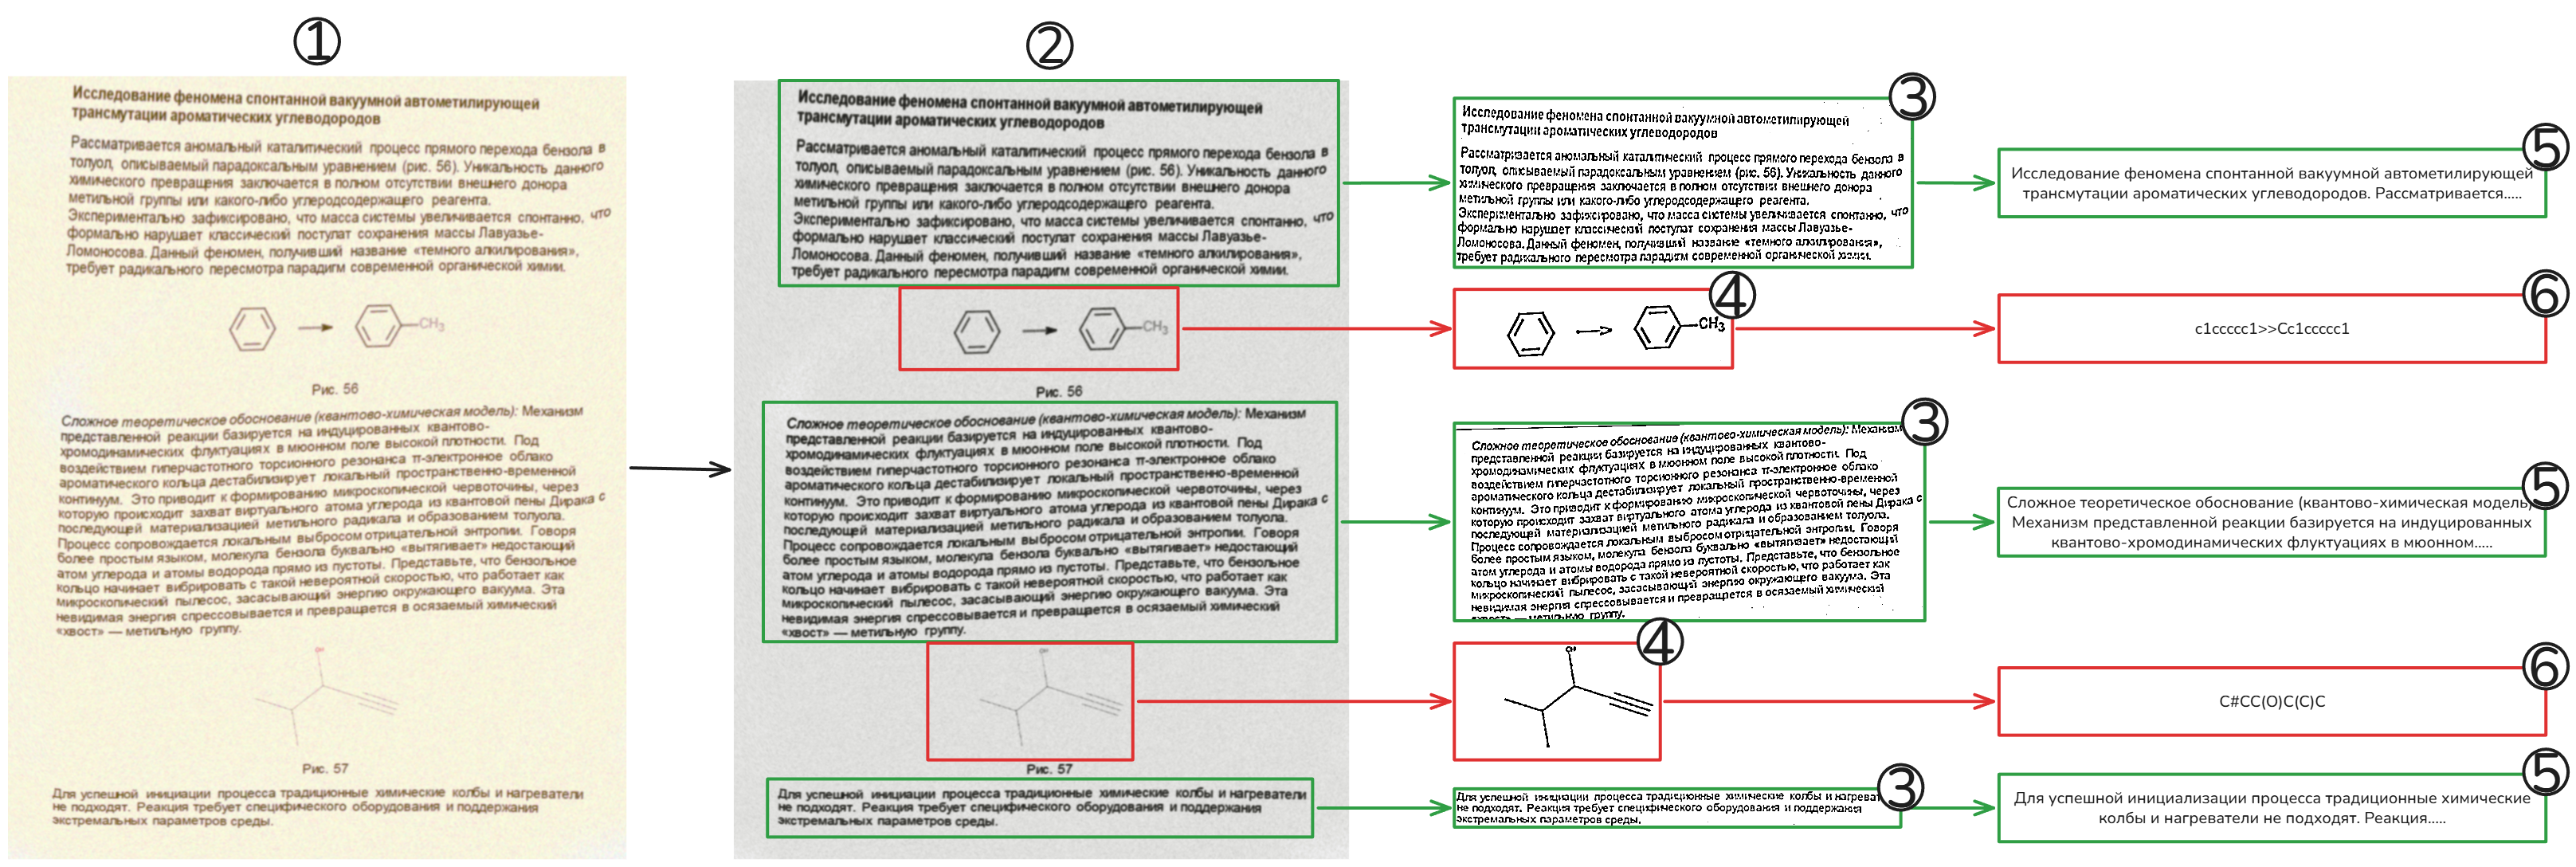
\includegraphics[width=0.9\textwidth]{example_prog.png}
\caption{End-to-end pipeline stages on a sample page: (1) original scanned page; (2) segmentation result with detected text and chemical blocks; (3) adaptively preprocessed text region; (4) adaptively preprocessed chemical formula; (5) extracted machine-readable text; (6) recognized chemical structure in SMILES format.}
\label{fig:pipeline_stages}
\end{figure*}

Fig.~\ref{fig:pipeline_stages} illustrates the end-to-end transformation of a scanned page through each pipeline stage, from raw image to structured text and SMILES output.

\subsection{RAG Retrieval Case Study: Pyrrole Synthesis}

To illustrate the practical utility of the proposed Dual-Stream RAG system, consider a complex user query: ``What are the synthesis conditions and structural intermediates for pyrrole derivatives in superbasic media?'' A standard keyword-based OCR search would miss the structural nuances hidden in historical diagrams.

When this query is processed, the system operates in parallel: the Text-Bibliographic stream searches the vector database (ChromaDB) and retrieves the exact historical text chunks describing the Trofimov reaction methodology---specifically the use of the KOH/DMSO catalytic superbasic system. Simultaneously, the Chemoinformatics stream retrieves the corresponding chemical graphs extracted via OCSR, yielding verified SMILES strings for both the intermediates (e.g., zwitterionic structures) and the final condensed products such as 4,5,6,7-tetrahydroindole (\texttt{C1CCC2=C(C1)C=CN2}).

The local LLM (YandexGPT 5 Lite) then integrates these two streams. Because the model is strictly grounded in the retrieved context, it generates a comprehensive, hallucination-free response that describes the synthesis pathway while providing the RDKit-validated structural codes, seamlessly integrating text and chemical topology.

\section{Experimental Validation}

To quantitatively validate the pipeline components, we conducted a controlled evaluation on a test set of 10 text-only page images and 20 chemical structure images (10 in detailed notation, 10 in skeletal notation). The goal was to measure the contribution of each processing stage and compare OCSR model performance under realistic scanning conditions.

\subsection{Text Recognition Accuracy}

OCR quality was measured using $1 - \text{WER}$ (Word Error Rate), which we favor over Character Error Rate (CER) because a single character substitution can alter the meaning of an entire chemical term, and WER better captures sentence-level semantic integrity. Six configurations were compared: baseline EasyOCR (OCR), with adaptive preprocessing (Pre), with LLM-based normalization (Norm), with heuristic normalization (NormE), and combined schemes.

\begin{table*}[t]
\centering
\small
\caption{OCR accuracy ($1 - \text{WER}$) across configurations. Best per row in bold.}
\label{tab:ocr}
\begin{tabular}{lcccccc}
\toprule
Test & OCR & +Pre & +Norm & +NormE & +Pre+NormE & \textbf{+Pre+Norm} \\
\midrule
1 & 0.1603 & 0.4737 & 0.5465 & 0.1603 & 0.4503 & \textbf{0.9394} \\
2 & 0.1742 & 0.5023 & 0.4838 & 0.1559 & 0.4909 & \textbf{0.8909} \\
3 & 0.2151 & 0.0154 & 0.3588 & 0.2000 & 0.0310 & \textbf{0.4113} \\
4 & 0.8734 & 0.8518 & 0.9240 & 0.8734 & 0.8500 & \textbf{0.9500} \\
5 & 0.6488 & 0.7610 & 0.8750 & 0.5780 & 0.7121 & \textbf{0.9212} \\
6 & 0.7091 & 0.6139 & 0.9643 & 0.7529 & 0.6450 & 0.8060 \\
7 & 0.2100 & 0.3986 & 0.3720 & 0.1995 & 0.4203 & \textbf{0.8711} \\
8 & 0.3656 & 0.0000 & 0.7923 & 0.3771 & 0.0000 & 0.0538 \\
9 & 0.7210 & 0.7812 & 0.8785 & 0.7494 & 0.8031 & \textbf{0.8976} \\
10 & 0.0636 & 0.3476 & 0.4295 & 0.0266 & 0.3523 & \textbf{0.9516} \\
\midrule
Mean & 0.4141 & 0.4746 & 0.6625 & 0.4073 & 0.4755 & \textbf{0.7693} \\
Std.~Dev. & 0.2936 & 0.2975 & 0.2460 & 0.3053 & 0.2935 & 0.2983 \\
\bottomrule
\end{tabular}
\end{table*}

Table~\ref{tab:ocr} shows that the combined configuration \textit{OCR+Pre+Norm} achieves the highest mean accuracy (0.7693). This represents an improvement of approximately 35 percentage points over the baseline. LLM-based normalization by itself (OCR+Norm) also performs well with the lowest standard deviation. Preprocessing alone provides modest gains, while heuristic normalization underperforms LLM-based correction.

\subsection{Chemical Structure Recognition Accuracy}

Each OCSR model was evaluated with and without adaptive preprocessing on both detailed and skeletal notations.

\begin{table*}[t]
\centering
\small
\caption{OCSR accuracy (correct/total) by model and notation type.}
\label{tab:ocsr}
\begin{tabular}{lcccccc}
\toprule
\multirow{2}{*}{Model} & \multicolumn{3}{c}{Without Preprocessing} & \multicolumn{3}{c}{With Preprocessing} \\
\cline{2-7}
 & Detailed & Skeletal & Total & Detailed & Skeletal & Total \\
\midrule
MolScribe & 8/10 & 10/10 & \textbf{18/20} & 5/10 & 9/10 & 14/20 \\
DECIMER & 2/10 & 4/10 & 6/20 & 4/10 & 2/10 & 6/20 \\
Qwen3-VL & 3/10 & 3/10 & 6/20 & 4/10 & 3/10 & 7/20 \\
\bottomrule
\end{tabular}
\end{table*}

As shown in Table~\ref{tab:ocsr}, MolScribe substantially outperforms the other models, achieving 18/20 without preprocessing and perfect recognition on skeletal formulas. Preprocessing did not universally improve OCSR quality: MolScribe's accuracy dropped after preprocessing, suggesting its native image handling is better suited to raw scans. DECIMER's total remained unchanged with a distribution shift, while Qwen3-VL showed a marginal improvement. These results confirm that MolScribe is the most reliable OCSR model for our archival corpus and guides our architectural choice in the pipeline.

\section{Hardware Acceleration and Local Deployment}

A core requirement of this architecture is complete local deployment to maintain data sovereignty. Processing multimodal VLM inference (Qwen3-VL), LLM text normalization (YandexGPT 5 Lite with LoRA adapters), and OCSR graph generation (MolScribe/DECIMER) concurrently requires significant computational resources.

The pipeline is optimized to run on a distributed local computing cluster equipped with high-performance consumer and workstation GPUs. The architecture efficiently balances VRAM loads across nodes featuring an NVIDIA RTX 3090 (24 GB), RTX 4070 Ti (12 GB), and RTX 3070 Ti (8 GB), supported by 96 GB of system RAM. This heterogeneous configuration allows the large context windows required by Qwen3-VL and the LLM to remain in memory, while OCSR inference is distributed across available devices. Batch processing of scanned books proceeds without external cloud dependencies, ensuring that sensitive chemical data never leaves the institutional network.

\section{Discussion and Limitations}

While the Dual-Stream pipeline effectively digitizes complex archives, several limitations remain.

First, the quantitative validation of individual pipeline components was conducted on a relatively modest dataset (30 images), reflecting the project's early stage. The observed trends--particularly the improvement of approximately 35 percentage points in OCR accuracy with LLM-based normalization and MolScribe's dominance for OCSR--are consistent enough to guide architectural decisions but should be confirmed on larger, more diverse collections.

Second, the lack of standardization in early 20th-century chemical drawings--varying line styles, non-standard abbreviations, and hand-drawn annotations--forces modern VLMs, trained predominantly on contemporary computer-rendered datasets, to occasionally misinterpret archaic notations. This is a fundamental domain shift problem that will require specialized fine-tuning data.

Third, the current heuristic page segmentation assumes a full-width horizontal block layout, limiting its applicability to multi-column journal layouts, side notes, or embedded tables. To address this, we are compiling an annotated dataset of historical multi-column journals to fine-tune YOLOv8 and Vision Transformer (ViT) models. This learned approach will robustly isolate text, tables, and chemical graphs prior to OCSR, improving adaptability to non-standard archival layouts.

Fourth, running advanced multimodal RAG locally imposes strict VRAM constraints. The concurrent execution of Qwen3-VL, YandexGPT 5 Lite, and OCSR models necessitates careful memory management and occasionally requires quantization techniques (e.g., 4-bit quantization of the LLM) that may slightly degrade reasoning capabilities. Future iterations will explore model distillation and optimized inference frameworks to alleviate this bottleneck.

\section{Conclusion}

We presented a sovereign, locally deployable architecture for the digitization of historical chemical literature, integrating adaptive preprocessing, Dual-Stream Retrieval (text and OCSR), and RAG with RDKit validation. By utilizing EasyOCR with LLM-based normalization for text and models such as MolScribe and Qwen3-VL for chemical graph translation, the system converts raw scans into structured, searchable information without relying on external cloud services or proprietary databases.

Applying this pipeline to the historical archives of the Siberian chemical school--the acetylene chemistry works of academicians Favorsky and Trofimov--demonstrated its capability to extract complex reaction pathways from degraded 20th-century publications. The mandatory RDKit validation step eliminates AI hallucinations at the chemical structure level, ensuring that the RAG database contains only scientifically sound representations. This architecture provides a secure foundation for bringing historical experimental chemistry into the modern data-driven era, enabling querying of both textual procedures and verified molecular structures from previously inaccessible archival documents.

\section*{Acknowledgment}

This work was supported by the state research project ``Development of Local Neural Network Architectures for Multimodal Knowledge Extraction (OCSR) and Semantic Analysis of Chemical Literature Using Large Language Models'' (No.~125122515025-5) and by the project ``Methods and Technologies for a Cloud Service-Oriented Digital Platform for the Collection, Storage, and Processing of Large Volumes of Multiformat Interdisciplinary Data and Knowledge Based on Artificial Intelligence, a Model-Driven Approach, and Machine Learning'' (FWEW-2021-0006).

\begin{thebibliography}{99}
\bibitem{ref1} A.~R.~Davletov, ``Modern methods of machine learning and OCR technology for automating document processing,'' \textit{Bulletin of Science}, no.~10(67), 2023. [Online]. Available: https://cyberleninka.ru/article/n/sovremennye-metody-mashinnogo-obucheniya-i-tehnologiya-ocr-dlya-avtomatizatsii-obrabotki-dokumentov

\bibitem{ref2} A.~V.~Kuchuganov, ``Methods and tools for semantic analysis and search of graphic information in document flow systems,'' Ph.D. dissertation, Izhevsk State Tech. Univ., 2015.

\bibitem{ref3} J.~Ha, R.~M.~Haralick, and I.~T.~Phillips, ``Recursive X-Y cut using bounding boxes of connected components,'' in \textit{Proc. 3rd Int. Conf. Document Analysis and Recognition}, 1995, vol.~2, pp.~952--955.

\bibitem{ref4} K.~Y.~Wong, R.~G.~Casey, and F.~M.~Wahl, ``Document analysis system,'' \textit{IBM J. Res. Develop.}, vol.~26, no.~6, pp.~647--656, 1982.

\bibitem{ref5} Z.~Shen \textit{et al.}, ``LayoutParser: a unified toolkit for deep learning based document image analysis,'' \textit{arXiv:2103.15348}, 2021.

\bibitem{ref6} B.~Wang \textit{et al.}, ``MinerU: an open-source solution for precise document content extraction,'' \textit{arXiv:2409.18839}, 2024.

\bibitem{ref7} Y.~Xu \textit{et al.}, ``LayoutLM: pre-training of text and layout for document image understanding,'' \textit{arXiv:1912.13318}, 2019.

\bibitem{ref8} Y.~Qian \textit{et al.}, ``MolScribe: robust molecular structure recognition with image-to-graph generation,'' \textit{arXiv:2205.14205}, 2022.

\bibitem{ref9} K.~Raja \textit{et al.}, ``DECIMER: deep learning for chemical image recognition,'' \textit{ResearchGate}, 2020.

\bibitem{ref10} O.~Kohulan \textit{et al.}, ``DECIMER.ai: an open platform for automated optical chemical structure identification, segmentation and recognition in scientific publications,'' \textit{J. Cheminform.}, vol.~15, p.~117, 2023.

\bibitem{ref11} Qwen Team, ``Qwen3-VL technical report,'' \textit{arXiv:2511.21631}, 2025.

\bibitem{ref12} H.~Liu \textit{et al.}, ``Visual instruction tuning,'' \textit{arXiv:2305.11845}, 2023.

\bibitem{ref13} Y.~Qian \textit{et al.}, ``RxnScribe: a sequence generation model for reaction diagram parsing,'' \textit{arXiv:2302.11894}, 2023.

\bibitem{ref14} X.~Zhong \textit{et al.}, ``Benchmarking retrieval-augmented generation for chemistry,'' \textit{arXiv:2505.07671}, 2025.

\bibitem{ref15} D.~Edge \textit{et al.}, ``From local to global: a graph RAG approach to query-focused summarization,'' \textit{arXiv:2404.16130}, 2024.
\bibitem{ref16} S.~Akhil, ``Overview of Tesseract OCR engine,'' 2016. [Online]. Available: https://www.researchgate.net/publication/315834331
\bibitem{ref17} ``Line-angle formula,'' Wikipedia. [Online]. Available: https://en.wikipedia.org/wiki/Skeletal\_formula
\bibitem{ref18} W.~A.~Warr, ``Representation of chemical structures,'' \textit{WIREs Comput. Mol. Sci.}, vol.~1, no.~4, pp.~557--579, 2011.
\bibitem{ref19} D.~Weininger, ``SMILES, a chemical language and information system. 1. Introduction to methodology and encoding rules,'' \textit{J. Chem. Inf. Comput. Sci.}, vol.~28, no.~1, pp.~31--36, 1988.
\bibitem{ref20} N.~M.~O'Boyle, ``Towards a universal SMILES representation,'' \textit{J. Cheminform.}, vol.~4, p.~22, 2012.
\bibitem{ref21} D.~Weininger \textit{et al.}, ``SMILES. 2. Algorithm for generation of unique SMILES notation,'' \textit{J. Chem. Inf. Comput. Sci.}, vol.~29, no.~2, pp.~97--101, 1989.
\bibitem{ref22} C.~Fifty \textit{et al.}, ``Context-aware molecular property prediction: a few-shot approach,'' \textit{arXiv:2002.08773}, 2020.
\end{thebibliography}

\end{document}
